% 2006_shanghai_liberal_q19_fig1: right triangular prism ABC-A1B1C1, angle ABC=90
% schematic oblique projection; topology from original PNG
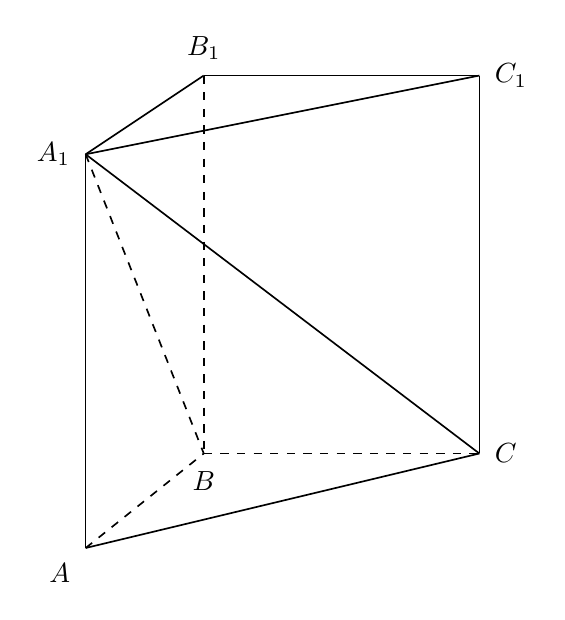
\begin{tikzpicture}[x=1cm,y=1cm,font=\normalsize,line width=.6pt]
\coordinate (A1) at (0,5);
\coordinate (B1) at (1.5,6);
\coordinate (C1) at (5,6);
\coordinate (A) at (0,0);
\coordinate (B) at (1.5,1.2);
\coordinate (C) at (5,1.2);
% visible prism edges (solid)
\draw[solid] (A1) -- (A);
\draw[solid] (A) -- (C);
\draw[solid] (C1) -- (C);
\draw[solid] (B1) -- (C1);
\draw[solid] (A1) -- (B1);
\draw[solid] (A1) -- (C1);
\draw[solid] (A1) -- (C);
% hidden prism edges (dashed)
\draw[dashed] (A) -- (B);
\draw[dashed] (B) -- (C);
\draw[dashed] (B1) -- (B);
\draw[dashed] (A1) -- (B);
% labels offset to avoid touching strokes
\node[left=2pt] at (A1) {$A_{1}$};
\node[above=2pt] at (B1) {$B_{1}$};
\node[right=2pt] at (C1) {$C_{1}$};
\node[below left=2pt] at (A) {$A$};
\node[below=3pt] at (B) {$B$};
\node[right=2pt] at (C) {$C$};
\end{tikzpicture}
